\documentclass[11pt]{article}

\usepackage[a4paper,margin=1in]{geometry}
\usepackage[T1]{fontenc}
\usepackage[utf8]{inputenc}
\usepackage{amsmath,amssymb,amsthm}
\usepackage{mathtools}
\usepackage{enumitem}
\usepackage{booktabs}
\usepackage{array}
\usepackage{tabularx}
\usepackage{xcolor}
\usepackage{algorithm}
\usepackage{algpseudocode}
\usepackage{graphicx}
\usepackage{hyperref}
\usepackage{cleveref}

\hypersetup{colorlinks=true,linkcolor=blue!50!black,citecolor=blue!50!black,urlcolor=blue!50!black}

\theoremstyle{plain}
\newtheorem{theorem}{Theorem}[section]
\newtheorem{lemma}[theorem]{Lemma}
\newtheorem{proposition}[theorem]{Proposition}
\newtheorem{corollary}[theorem]{Corollary}
\theoremstyle{definition}
\newtheorem{definition}[theorem]{Definition}
\newtheorem{example}[theorem]{Example}
\theoremstyle{remark}
\newtheorem{remark}[theorem]{Remark}

\crefname{theorem}{Theorem}{Theorems}
\crefname{lemma}{Lemma}{Lemmas}
\crefname{proposition}{Proposition}{Propositions}
\crefname{corollary}{Corollary}{Corollaries}
\crefname{definition}{Definition}{Definitions}
\crefname{remark}{Remark}{Remarks}

\newcommand{\CP}{\mathbb{CP}}
\newcommand{\R}{\mathbb{R}}
\newcommand{\C}{\mathbb{C}}
\newcommand{\type}{\mathrm{type}}
\newcommand{\level}{\mathrm{level}}
\newcommand{\msplit}{\mathrm{split}}
\newcommand{\link}{\mathrm{link}}
\newcommand{\weld}{\mathrm{weld}}
\newcommand{\st}{\mathrm{st}}
\newcommand{\col}{\mathfrak{c}}
\newcommand{\todo}[1]{\textcolor{red!70!black}{\textsf{[TODO: #1]}}}
\setlength{\emergencystretch}{2em}
\newcolumntype{L}{>{\raggedright\arraybackslash}X}

\title{\bf Stellar Subdivision Schemes on Balanced Triangulations:\\
Pointerless Maubach Bisection and Riemann Surfaces in $\CP^2$}
\author{Vin\'icius Moreira Mello\\[2pt]
{\small Departamento de Matem\'atica, Universidade Federal da Bahia, Salvador, Brazil}\\
{\small\texttt{vinicius.mello@ufba.br}}}
\date{Draft -- \today}

\begin{document}
\maketitle

\begin{abstract}
We revisit newest-vertex (Maubach) bisection from a purely combinatorial
standpoint. Following the framework of \emph{stellar subdivision
schemes}, a scheme is a pair formed by a combinatorial invariant on
ordered simplicial meshes and a subdivision algorithm that provably preserves it,
stated and proved level by level through ordered stellar operations alone. In this
language, the facet-based scheme of Mitchell and the edge-based scheme of
Maubach have the same deductive structure. We then study which
\emph{initial} meshes a scheme can start from. For Maubach's scheme, the
strong form of the invariant on a conforming mesh is equivalent to the
mesh being \emph{balanced}, i.e.\ properly $(n{+}1)$-colorable. This places
the classical constructions (products of simplices, barycentric
subdivisions) and the recent coloring-based initializations in a single
picture, and it applies verbatim to triangulations of \emph{closed
manifolds}, a setting absent from the finite-element literature. As a case
study we show that Gaifullin's 15-vertex triangulation of $\CP^2$ is
balanced, and hence, by Gaifullin's minimality theorem, a vertex-minimal
balanced triangulation of $\CP^2$, while Kühnel's 9-vertex $\CP^2_9$ is
not. Balance is also exactly what makes Atalay and Mount's pointerless LPT
codes portable. Every seed cell, ordered by color, is a copy of the Kuhn
reference simplex. Whether a facet lies on the seed boundary is decided by
one table lookup and one integer comparison, and the neighbor across it
is the same code in the adjacent seed cell. A seed index and a seed
adjacency table therefore suffice to run pointerless, conforming Maubach
bisection over any balanced seed, with no floating point. We
illustrate the whole construction by triangulating smooth plane algebraic
curves, i.e.\ compact Riemann surfaces, as codimension-2 loci
\emph{intrinsically} inside $\CP^2$, by a continuation algorithm driven
entirely by the combinatorial neighbor relations of the pointerless mesh.
\end{abstract}

\tableofcontents

% =====================================================================
\section{Introduction}
\label{sec:intro}
% =====================================================================

Adaptive refinement of simplicial meshes by \emph{bisection} is one of the
oldest tools of computational geometry and numerical analysis. Among the
many variants, newest-vertex bisection in the form given by
Maubach~\cite{maubach1995} and Traxler~\cite{traxler1997} stands out in
arbitrary dimension $n$. It is \emph{blind}, meaning the bisection edge of a
cell is determined by combinatorial data alone. It is conforming and
produces at most $n\,n!\,2^{n-2}$ similarity classes per initial simplex~\cite{amp2000}. It
also admits optimal closure estimates~\cite{bdd2004,stevenson2008}. Its one
well-known weakness is the initial mesh: the method only works if the
vertices of the initial cells are ordered \emph{compatibly}. For $n\ge3$
such orderings do not exist for every mesh, and a substantial literature
addresses how to repair
this~\cite{kossaczky1994,stevenson2008,agk2018,belda2023,dgs2025}.

This paper has three strands.

\paragraph{1. Stellar subdivision schemes.}
The author's thesis~\cite{mello2006}, available only in Portuguese,
developed a framework in which a \emph{subdivision scheme} is a pair: a
set of combinatorial invariants on ordered simplicial meshes, and an
algorithm $\mathrm{Subdivide}(K,\sigma)$ that propagates ordered stellar
subdivisions until $\sigma$ can be split without violating the invariants.
Correctness is proved by a short induction on the hierarchy level, using
only the face operators $\partial_i$ of the ordered mesh. The framework
covers Mitchell's facet-based scheme~\cite{mitchell1991} and Maubach's
edge-based scheme with the same deductive skeleton. We present it here in
English, in a self-contained way (\Cref{sec:stellar,sec:maubach}).

\paragraph{2. Initial meshes.}
We show that, on conforming meshes, the strong form of Maubach's invariant
(``every shared facet sits at the same local index on both sides'') is
equivalent to the mesh being \emph{balanced} in the sense of Stanley,
i.e.\ admitting a proper vertex coloring by $n+1$ colors
(\Cref{prop:strong-balanced}). The thesis's two constructions, the
canonical triangulation of a product of simplices and the barycentric
subdivision, become one-line corollaries. So does a product construction
for already-balanced meshes. This is the $N=n$ case of the recent
coloring-based initialization of Diening, Gehring and Storn~\cite{dgs2025},
and is equivalent to Traxler's reflected-partition
condition~\cite{traxler1997}. What seems new is its use on
\emph{closed-manifold seeds}. We prove that Gaifullin's 15-vertex
triangulation of $\CP^2$~\cite{gaifullin2009} is balanced, and deduce from
Gaifullin's own minimality theorem that no balanced triangulation of
$\CP^2$ has fewer vertices (\Cref{thm:gaifullin}). Kühnel's 9-vertex
$\CP^2_9$~\cite{kuhnelbanchoff1983} is not balanced
(\Cref{prop:kuhnel}).

\paragraph{3. Pointerless codes.}
Atalay and Mount's LPT codes~\cite{atalaymount2007} represent a Maubach
hierarchy over a Kuhn-triangulated cube with no pointers at all. Geometry
and neighbors of a cell are computed from a small integer code. We show
that the only feature of the cube their neighbor rules really use is
balance. Consequently, the codes extend to any balanced seed mesh by
adding a seed index and a seed adjacency table. The seed-boundary test
reduces to a precomputed table plus one comparison of orthant
coordinates, and crossing into the next seed cell keeps the code
unchanged (\Cref{sec:lpt}). We also quantify why codes matter: the
storage of an explicit incidence structure grows roughly by a factor
$1.6$ per dimension, and it is already $11$ times that of the codes
for $d=4$.

\paragraph{Application.}
We combine the three strands to triangulate a smooth projective plane curve
$\{F=0\}\subset\CP^2$, a compact Riemann surface, directly as a
codimension-2 submanifold of the real 4-manifold $\CP^2$. We seed with
Gaifullin's triangulation, refine by pointerless Maubach bisection along
Fubini--Study geodesics, and follow the curve by a continuation algorithm
that uses only the mesh's combinatorial neighbor queries
(\Cref{sec:riemann}). Unlike chart- or branch-cut-based approaches, the
construction is intrinsic: points at infinity play no special role.

\paragraph{Contributions.}
\begin{enumerate}[itemsep=2pt]
\item An English, self-contained account of stellar subdivision schemes and of
  Maubach's scheme within them. It includes an invariant that is
  preserved at every level of the hierarchy, and its precise relation to
  Stevenson's matching condition (\Cref{sec:stellar,sec:maubach}).
\item The equivalence ``strongly Maubach-compatible $\iff$ balanced'' for
  conforming meshes, a counterexample showing that index-only matching is
  insufficient, and closure of balance under products
  (\Cref{sec:initial}).
\item Balanced seeds for closed manifolds. Gaifullin's triangulation is a
  vertex-minimal balanced triangulation of $\CP^2$
  (\Cref{thm:gaifullin}).
\item An extension of LPT codes to arbitrary balanced seeds. It has a
  fully combinatorial neighbor procedure: an $O(1)$ table-based
  seed-boundary test and same-code seed crossing. It comes with a graded,
  conforming leaf-set data structure and a quantitative comparison with
  explicit incidence storage (\Cref{sec:lpt}).
\item An intrinsic, adaptive triangulation algorithm for Riemann surfaces
  in $\CP^2$ based on combinatorial continuation, with measurements
  (\Cref{sec:riemann}).
\end{enumerate}

\Cref{sec:related} reviews related work and states how our approach
compares.

% =====================================================================
\section{Related work}
\label{sec:related}
% =====================================================================

\paragraph{Bisection and initial meshes.}
Longest-edge bisection goes back to Rivara~\cite{rivara1984,rivara1991}.
Newest-vertex bisection (NVB) was introduced in 2D by
Mitchell~\cite{mitchell1988,mitchell1991}, extended to 3D by
Bänsch~\cite{bansch1991} and Kossaczký~\cite{kossaczky1994}, and to
arbitrary dimension by Maubach~\cite{maubach1995} and
Traxler~\cite{traxler1997}. Arnold, Mukherjee and Pouly~\cite{amp2000}
proposed a marked variant for tetrahedra that accepts any initial mesh.
Binev, Dahmen and DeVore~\cite{bdd2004} and Stevenson~\cite{stevenson2008}
proved the closure estimates that underlie optimality of adaptive finite
elements. All of these methods constrain the initial mesh.
\begin{itemize}[itemsep=1pt]
\item Traxler's \emph{reflected} condition requires the ordered vertex
  lists of neighbors to differ in exactly one position. On a simply
  connected domain it holds iff every interior $(n{-}2)$-face has even
  degree.
\item Stevenson's weaker \emph{matching-neighbour} condition is
  necessary and sufficient for all uniform refinements to be conforming.
  Whether every 3D mesh admits it is open. Following
  Kossaczký, Stevenson therefore pre-refines every simplex into $\frac12(n{+}1)!$ pieces.
\item Alkämper, Gaspoz and Klöfkorn~\cite{agk2018} give an $O(n)$
  renumbering guaranteeing termination.
\item Belda-Ferrín et al.~\cite{belda2018,belda2022,belda2023} perform $n$
  marked-bisection stages before switching to Maubach, and note that for
  $n>3$ ``there is not any known method to extract a reflection structure
  from an arbitrary unstructured conformal mesh''.
\item Diening, Gehring and Storn~\cite{dgs2025} initialize Maubach's
  routine from a proper $(N{+}1)$-coloring of the vertices, with $N\ge n$,
  computed greedily in linear time. When $N>n$ each cell is treated as a
  face of a virtual $N$-simplex. They prove shape regularity and the
  closure estimate. For $N=n$ their condition is Traxler's; see
  also~\cite{dst2023,gehring2023}.
\end{itemize}
All of the above concern triangulations of domains in $\R^n$.

Our treatment differs from this literature in two respects. First, the
compatibility condition is formulated as an \emph{invariant}, hereditary
in the level, rather than as a condition on the initial mesh only.
Second, we apply it to seeds that triangulate closed manifolds. The
equivalence of \Cref{prop:strong-balanced} makes the connection with the
coloring viewpoint of~\cite{traxler1997,dgs2025} explicit.

\paragraph{Stellar theory and balanced complexes.}
Stellar subdivisions and welds go back to Alexander and Newman;
see~\cite{lickorish1999} for a modern account. In geometry processing,
Velho's stellar subdivision grammars~\cite{velho2003} and $4$--$8$
meshes~\cite{velhozorin2001} describe adaptive surface refinement by
stellar operations; $4$--$8$ refinement is NVB in two dimensions. A
$d$-complex is \emph{balanced} if its graph is $(d{+}1)$-colorable.
Joswig~\cite{joswig2002} characterized balanced complexes through their
group of projectivities. Izmestiev, Klee and Novik~\cite{ikn2017}
introduced cross-flips, the balanced analogue of bistellar moves.
Venturello~\cite{venturello2019} found small balanced triangulations of
several manifolds. We are not aware of work connecting balanced
triangulations of closed manifolds with bisection refinement.

\paragraph{Pointerless hierarchical meshes.}
Several representations encode a simplex of a regular bisection hierarchy
by a label rather than by pointers:
\begin{itemize}[itemsep=1pt]
\item Hebert~\cite{hebert1994}, Evans, Kirkpatrick and
  Townsend~\cite{ekt2001}, and Lee, De Floriani and Samet~\cite{ldfs2001},
  in 2D and 3D;
\item Maubach's own neighbor location scheme~\cite{maubach1996};
\item Atalay and Mount's LPT codes~\cite{atalaymount2007}, in arbitrary
  dimension over a Kuhn-triangulated cube, which we previously
  re-implemented to generate adaptive cellular infill structures for 3D
  printing~\cite{sa2015adaptive};
\item Weiss and De Floriani's diamond hierarchies~\cite{weissdefloriani2011},
  which use the star of the bisection edge as primitive;
\item Dupuy's concurrent binary trees~\cite{dupuy2020}, which implement
  longest-edge bisection on the GPU;
\item Boissonnat, Kachanovich and Wintraecken's permutahedral
  encoding of
  Freudenthal--Kuhn simplices~\cite{bkw2023}, which is compact but not
  adaptive.
\end{itemize}
The closest architectural analogue of our construction is the
\emph{forest} approach of p4est~\cite{p4est2011} and
t8code~\cite{bursteddeholke2016}. There, an arbitrary coarse mesh is
refined tree by tree, with a per-tree linear code and an inter-tree
connectivity table. Those forests are \emph{non-conforming}: they allow
hanging nodes and use red refinement in 2D and 3D. Ours is a conforming,
graded bisection forest in arbitrary dimension.

\paragraph{Riemann surfaces and implicit manifolds.}
Numerical approaches to compact Riemann surfaces work with a branched
covering of $\CP^1$ and compute analytic invariants such as monodromy and
period matrices~\cite{deconinckvanhoeij2001,bobenkoklein2013,kranich2016}.
Visualizations use parametrizations~\cite{hanson1994} or multivalued graphs
over $\C$ with branch cuts~\cite{nieser2010}. Our construction is a
simplicial complex of the curve inside $\CP^2$ itself.

Piecewise-linear approximation of implicit manifolds of arbitrary
codimension over Freudenthal--Kuhn triangulations goes back to
Allgower
and Schmidt~\cite{allgowerschmidt1985,allgowergeorg2003}. Other related
constructions are:
\begin{itemize}[itemsep=1pt]
\item Weigle and Banks~\cite{weiglebanks1996} extract the zero set of a
  function $\C^2\to\C$ as a surface in $\R^4$ on a uniform grid. This is
  the closest predecessor of our codimension-2 extraction, but it works in
  an affine chart.
\item Castelo et al.~\cite{castelo2006} give an adaptive triangulation in
  any dimension for implicit manifolds.
\item Boissonnat, Kachanovich and Wintraecken~\cite{bkw2023} trace
  isomanifolds cell by cell from a seed point over uniform
  Coxeter--Freudenthal--Kuhn triangulations, with guarantees of
  topological correctness~\cite{boissonnatwintraecken2022}. Our
  continuation follows the same strategy, over an adaptive mesh of a
  compact manifold, but without certification.
\item Certified alternatives exist for curves and surfaces in low
  dimension: interval-based subdivision~\cite{plantingavegter2004},
  Bernstein subdivision~\cite{mourrainpavone2009,reuter2008}, and
  numerical cell decomposition~\cite{bertinireal2017}.
\item Bisection hierarchies are also used for isosurface extraction in
  $\R^3$~\cite{gerstnerrumpf2000,pascucci2002,ju2024}.
\end{itemize}

% =====================================================================
\section{Ordered meshes and stellar subdivision schemes}
\label{sec:stellar}
% =====================================================================

\subsection{Ordered simplicial complexes and conforming meshes}

\begin{definition}
An \emph{ordered simplicial complex} $K$ on a finite vertex set $V$ is an
abstract simplicial complex together with a partial order $<$ on $V$
such that the vertices of every simplex are totally ordered. We write
$\sigma=\langle v_0,\dots,v_n\rangle$ with $v_0<\dots<v_n$ and $\sigma[j]=v_j$.
The \emph{face operators} $\partial_i:K_n\to K_{n-1}$ delete the $i$-th
vertex. They satisfy $\partial_j\partial_i=\partial_{i-1}\partial_j$ for
$j<i$. More generally, for $0\le j_0<\dots<j_k\le n$ we write
$\sigma[j_0,\dots,j_k]:=\langle v_{j_0},\dots,v_{j_k}\rangle$.
\end{definition}

Equalities such as $\partial_i\sigma=\partial_j\omega$ are equalities of
\emph{ordered} simplices. This will matter in \Cref{rem:index-only}. The
order encodes, locally, everything the subdivision algorithms need. No
geometric information is ever consulted.

For an $m$-dimensional complex, $m$-simplices are \emph{cells} and
$(m{-}1)$-simplices are \emph{facets}. $K$ is a \emph{pseudomanifold} if it
is pure and every facet lies in at most two cells. The \emph{dual graph}
$G(K)$ has the cells as nodes and the facets shared by two cells as edges.
$K$ is \emph{strongly connected} if $G(K)$ is connected.

\begin{definition}[\cite{mello2006}]
A strongly connected pseudomanifold $K$ is \emph{hereditary} if the star
$\st(v,K)$ of every vertex is strongly connected. A hereditary
pseudomanifold is called a \emph{conforming mesh}.
\end{definition}

In a conforming mesh the star of every simplex is strongly connected.
The star of any face can therefore be traversed by walking across facets,
which is how the algorithms below find cells.

\subsection{Ordered stellar subdivisions}

Let $\delta\in K$ and $v\notin V$. The \emph{stellar subdivision} $K'=K(\delta,v)$
replaces $\st(\delta,K)$ by $v\star\partial\delta\star\link(\delta,K)$. We
write $K'=K(\delta,v)_l$, an \emph{ordered stellar subdivision}, when the
order on $V\cup\{v\}$ places $v$ at position $l$ in every cell of
$\st(v,K')$.

Let $\sigma$ be an $m$-cell and $\delta=\sigma[j_0,\dots,j_n]$ one of its
faces. Applying $(\delta,v)_l$ to $\sigma$ yields $n+1$ \emph{children}
$c_0\sigma,\dots,c_n\sigma$, one for each facet of $\partial\delta$. They
can be indexed so that
\begin{equation}\label{eq:children}
  \partial_l\,c_i\sigma=\partial_{j_{n-i}}\,\sigma,
\end{equation}
and orientations then propagate by $o(c_i\sigma)=o(\sigma)(-1)^{l+j_{n-i}}$.

A sequence of ordered stellar subdivisions starting from a mesh $K$ induces a
hierarchy on cells. Let $\level(\sigma)=0$ for $\sigma\in K$ and
$\level(c_i\sigma)=\level(\sigma)+1$. Every cell $\sigma$ of positive level
has a unique \emph{parent} $p(\sigma)$ and a unique \emph{weld vertex}
$\weld(\sigma)\in\sigma\setminus p(\sigma)$, the vertex whose removal by a
stellar weld would undo the subdivision that created $\sigma$.

\subsection{Subdivision schemes}

\begin{definition}[\cite{mello2006}]
A \emph{stellar subdivision scheme} is a pair $(\mathcal I,\mathrm{Subdivide})$.
Here $\mathcal I$ is a set of invariants referring only to combinatorial
data of a conforming mesh: vertex order, adjacency, $\level$, and possibly
labels with prescribed behavior under subdivision. Given a mesh $K$
satisfying $\mathcal I$ and a cell $\sigma$, the algorithm
$\mathrm{Subdivide}(K,\sigma)$ applies a sequence of ordered star
subdivisions $(\delta_1,v_1)_{l_1}\cdots(\delta_q,v_q)_{l_q}$ in which only
$\delta_q$, the \emph{subdivision face}, is a face of $\sigma$. The
result, and every intermediate mesh, must again satisfy $\mathcal I$.
\end{definition}

A typical invariant bounds the level jump across facets:
\begin{equation}\tag{OneLevel}
  \partial_i\sigma=\partial_j\omega\;\Longrightarrow\;|\level(\sigma)-\level(\omega)|\le1 .
\end{equation}

The thesis names three desirable properties of $\mathrm{Subdivide}$. To
avoid a clash with \emph{balanced complexes} (\Cref{sec:initial}), we
rename the third property here. $\mathrm{Subdivide}$ is:
\begin{itemize}[itemsep=2pt]
\item \emph{consistent}, if there is a function $\msplit$ assigning each
  cell $\sigma'$ a face $\msplit(\sigma')\subset\sigma'$ such that every
  cell in the star of a subdivided face $\delta$ has
  $\msplit(\sigma')=\delta$. All cells split in one stellar operation
  agree on what to split, and a generic weld algorithm can undo the
  refinement;
\item \emph{alternating}, if $\weld(\sigma)\notin\msplit(\sigma)$ for
  every cell. Newly created faces are never immediately split, which
  forces propagation outward;
\item \emph{level-homogeneous} (``balanced'' in~\cite{mello2006}), if all
  cells in the star of a subdivided face have the same level.
\end{itemize}

\subsection{Mitchell's scheme}
\label{sec:mitchell}

Mitchell's scheme always splits the facet opposite the first vertex,
$\msplit(\sigma):=\partial_0\sigma$. Written as invariants, this becomes
the following definition.

\begin{definition}[Mitchell invariants]
$K$ satisfies the \emph{Mitchell invariants} if it satisfies (OneLevel)
and, for adjacent cells with $\partial_i\sigma=\partial_j\omega$,
\begin{align*}
  \level(\sigma)=\level(\omega)&\;\Longrightarrow\; i=0=j\ \text{ or }\ i\ne0\ne j, \tag{MitchellA}\\
  \level(\sigma)=\level(\omega)+1&\;\Longrightarrow\; i=0\ne j. \tag{MitchellB}
\end{align*}
\end{definition}

(MitchellA) says two same-level neighbors either share their split facet
or neither contains the other's. (MitchellB) says that splitting the
coarser cell hands the split facet to one of its children. Any mesh
satisfies the invariants after the ordered cone $(\sigma,v_\sigma)_0$ is
applied to every cell. The algorithm is two lines: if the neighbor across
$\partial_0\sigma$ is coarser, subdivide it first; then split
$\partial_0\sigma$ at position $0$.

\begin{theorem}[\cite{mello2006}]\label[theorem]{thm:mitchell}
Mitchell's algorithm preserves the Mitchell invariants and is consistent,
alternating and level-homogeneous.
\end{theorem}

The proof uses three lemmas that recur, in the same roles, for Maubach's
scheme:
\begin{itemize}[itemsep=1pt]
\item a \emph{direction lemma} saying which neighbor can be coarser;
\item a \emph{child lemma} describing the adjacencies among the children
  of a single split cell;
\item a \emph{two-cell lemma} showing the invariants survive splitting one
  of two adjacent cells.
\end{itemize}
The induction on $\level(\sigma)$ then assembles them. We give the
Maubach versions in full below. The Mitchell versions are simpler.

% =====================================================================
\section{Maubach's scheme}
\label{sec:maubach}
% =====================================================================

Maubach's scheme splits an \emph{edge}. For an $m$-dimensional mesh set
\[
  \type(\sigma):=m-(\level(\sigma)\bmod m)\in\{1,\dots,m\},\qquad
  \msplit(\sigma):=\sigma[0,\type(\sigma)] .
\]
The new vertex is inserted at position $\type(\sigma)$. By
\eqref{eq:children}, the two children of
$\sigma=\langle v_0,\dots,v_m\rangle$ under $(\sigma[0,l],v)_l$, with
$l=\type(\sigma)$, are
\[
  c_0\sigma=\langle v_0,\dots,v_{l-1},v,v_{l+1},\dots,v_m\rangle,\qquad
  c_1\sigma=\langle v_1,\dots,v_l,v,v_{l+1},\dots,v_m\rangle .
\]
This is exactly the rule of~\cite{maubach1995}, and of \cite[Alg.~1]{dgs2025}.

\begin{definition}[Maubach invariants]\label[definition]{def:maubach}
The mesh $K$ satisfies the \emph{Maubach invariants} if it satisfies
(OneLevel) and,
for adjacent cells with $\partial_i\sigma=\partial_j\omega$,
\begin{align*}
  \level(\sigma)=\level(\omega)&\;\Longrightarrow\; i=j\ \text{ or }\ \{i,j\}=\{0,\type(\omega)\},\tag{MaubachA}\\
  \level(\sigma)=\level(\omega)+1&\;\Longrightarrow\; i=\type(\omega)\ \text{ and }\ j\in\{0,\type(\omega)\}.\tag{MaubachB}
\end{align*}
We say $K$ is \emph{strongly compatible} if $\partial_i\sigma=\partial_j\omega\Rightarrow i=j$ for all
adjacent cells. At level $0$ this implies the Maubach invariants.
\end{definition}

(MaubachA) implies that two same-level neighbors either share their split
edge or neither contains the other's. Indeed, if $\msplit(\sigma)\subset\omega$
then $i\notin\{0,\type\}$, so $i=j$ and the two cells differ in a single
vertex away from the split edge. (MaubachB) implies that splitting the
coarser cell gives one of its children exactly the facet the finer
neighbor already has.

\begin{lemma}[direction]\label[lemma]{lem:direction}
If $K$ satisfies the Maubach invariants and $\partial_i\sigma=\partial_j\omega$, then
$\level(\omega)\le\level(\sigma)$ when $i\notin\{0,\type(\sigma)\}$, and
$\level(\omega)\ge\level(\sigma)$ when $i\in\{0,\type(\sigma)\}$.
Moreover, $\level(\omega)<\level(\sigma)$ implies $i=\type(\omega)$.
\end{lemma}

\begin{proof}
If $\level(\omega)>\level(\sigma)$ then $\level(\omega)=\level(\sigma)+1$
by (OneLevel). (MaubachB), with the roles of the cells exchanged, gives
$i\in\{0,\type(\sigma)\}$. If $\level(\omega)<\level(\sigma)$, then
(MaubachB) gives $i=\type(\omega)$. Since $\type(\omega)\ne\type(\sigma)$
and $\type\ne0$, it follows that $i\notin\{0,\type(\sigma)\}$.
\end{proof}

\begin{lemma}[children]\label[lemma]{lem:children}
For a single cell $\omega$ and $l>0$, the children of $(\omega[0,l],v)_l$
satisfy $\partial_0c_0\omega=\partial_{l-1}c_1\omega$.
\end{lemma}

\begin{proof}
Both sides equal $\langle v_1,\dots,v_{l-1},v,v_{l+1},\dots,v_m\rangle$.
\end{proof}

\begin{lemma}[two cells]\label[lemma]{lem:twocells}
Let $K$ consist of two adjacent cells with $\partial_i\sigma=\partial_j\omega$ and
$0\le\level(\sigma)-\level(\omega)\le1$, satisfying the Maubach invariants.
Then $K(\omega[0,l],v)_l$, with $l=\type(\omega)$, satisfies them as well.
\end{lemma}

\begin{proof}
There are seven cases. They are distinguished by whether the levels are
equal or differ by one, and by which of $i,j$ lie in $\{0,l\}$. In each
case, \Cref{lem:children} settles the pair $c_0\omega,c_1\omega$. The
remaining relation involving $\sigma$ reduces to a single facet identity:
\begin{center}
\small
\begin{tabular}{@{}clll@{}}
\toprule
& levels & indices & resulting relation \\
\midrule
1 & equal & $i=j=0$ & $\partial_0\sigma=\partial_l c_1\omega$ \hfill (MaubachB)\\
2 & equal & $i=j=l$ & $\partial_l\sigma=\partial_l c_0\omega$ \hfill (MaubachB)\\
3 & equal & $i=j=k\notin\{0,l\}$ & $\sigma$ is split too; $\partial_k c_0\sigma=\partial_k c_0\omega$, $\partial_{k-1}c_1\sigma=\partial_{k-1}c_1\omega$ \hfill (MaubachA)\\
4 & equal & $i=0,\ j=l$ & $\partial_0\sigma=\partial_l c_0\omega$ \hfill (MaubachB)\\
5 & equal & $i=l,\ j=0$ & $\partial_l\sigma=\partial_l c_1\omega$ \hfill (MaubachB)\\
6 & $+1$ & $i=l,\ j=0$ & $\partial_l\sigma=\partial_l c_1\omega$ \hfill (MaubachA)\\
7 & $+1$ & $i=l,\ j=l$ & $\partial_l\sigma=\partial_l c_0\omega$ \hfill (MaubachA)\\
\bottomrule
\end{tabular}
\end{center}
In cases 1--5, $\sigma$ becomes one level coarser than the children of
$\omega$, and (MaubachB) applies. In cases 6--7 the levels become equal
and (MaubachA) applies.
\end{proof}

\begin{algorithm}[t]
\caption{$\textsc{MaubachSubdivide}(K,\sigma)$~\cite{mello2006}}
\label{alg:maubach}
\begin{algorithmic}[1]
\Require conforming mesh $K$ satisfying the Maubach invariants; cell $\sigma$
\State $k\gets\type(\sigma)$; $\mathit{st}\gets[\,]$; $Q\gets(\sigma)$
\While{$Q\neq\varnothing$}
  \State $c\gets\mathrm{pop}(Q)$
  \If{$c$ not visited}
    \State mark $c$ visited; append $c$ to $\mathit{st}$
    \For{$i\in\{0,\dots,m\}\setminus\{0,k\}$} \Comment{facets containing the split edge}
      \State $c_a\gets\mathrm{adjacent}(c,i)$
      \If{$c_a$ not visited}
        \If{$\level(c_a)<\level(c)$}
          \State $\textsc{MaubachSubdivide}(K,c_a)$; $c_a\gets\mathrm{adjacent}(c,i)$
        \EndIf
        \State push $c_a$ onto $Q$
      \EndIf
    \EndFor
  \EndIf
\EndWhile
\State split the edge $\sigma[0,k]$ at position $k$ in every cell of $\mathit{st}=\st(\sigma[0,k],K)$
\end{algorithmic}
\end{algorithm}

\begin{theorem}[\cite{mello2006}]\label[theorem]{thm:maubach}
If $K$ satisfies the Maubach invariants, so does the result of
\Cref{alg:maubach} applied to any cell. The algorithm is consistent,
alternating and level-homogeneous.
\end{theorem}

\begin{proof}
The proof is by induction on $\level(\sigma)$. Suppose $\sigma$ has the
minimal level in $K$. By \Cref{lem:direction}, every cell sharing the
split edge $\epsilon$ has the same level, so the recursive call never
fires. The loop then walks $\st(\epsilon,K)$, which is possible because
$K$ is conforming. By (MaubachA) every cell in the star has split edge
$\epsilon$, which gives consistency and level-homogeneity.
\Cref{lem:twocells}, applied to every adjacent pair meeting the star,
preserves the invariants. For higher levels, \Cref{lem:direction} and the
induction hypothesis applied to the recursive call reduce to the base
case.
\end{proof}

\subsection{Relation to Traxler and Stevenson}
\label{sec:stevenson}

Traxler~\cite{traxler1997} and Stevenson~\cite{stevenson2008} constrain
only the initial mesh, and then prove that all uniform refinements are
conforming~\cite[Thm.~4.3]{stevenson2008}. Stevenson uses Traxler's
convention. A tagged simplex $(x_0,\dots,x_n)_\gamma$ is bisected along
$x_0x_n$, and $T_R=(x_n,x_1,\dots,x_\gamma,x_{n-1},\dots,x_{\gamma+1},x_0)_\gamma$
denotes the tagged simplex with the same children. Two neighbors are
\emph{reflected} if the vertex sequence of $T$ or of $T_R$ agrees with
that of $T'$ in all but one position. His condition~(b) on the initial
mesh has two clauses:
\begin{itemize}[itemsep=1pt]
\item if the refinement edge of either cell lies on the common facet, the
  two cells are reflected neighbors;
\item otherwise, their neighboring children are.
\end{itemize}
At level $0$, Traxler's type $\gamma=0$ with a given vertex order
corresponds to Maubach's type $n$ with the same order~\cite[Rem.~4]{dgs2025}.
In both cases the refinement edge is the first--last pair.

\begin{proposition}\label[proposition]{prop:stevenson}
Let $K$ be a level-$0$ mesh satisfying (MaubachA). For adjacent cells
$\sigma,\omega$:
\begin{enumerate}[label=(\alph*),itemsep=1pt]
\item if $\partial_i\sigma=\partial_i\omega$, their vertex sequences
  agree in all but position $i$;
\item if $\partial_0\sigma=\partial_n\omega$, neither refinement edge lies
  on the common facet, and the children containing the common facet
  have vertex sequences that agree in all but one position.
\end{enumerate}
Hence (MaubachA) at level $0$ implies the analogue of Stevenson's
condition~(b), with $T$ always used in place of $T_R$.
\end{proposition}

\begin{proof}
(a) is immediate from the definition. For (b), write
$\sigma=\langle a,f_1,\dots,f_n\rangle$ and
$\omega=\langle f_1,\dots,f_n,b\rangle$. The refinement edges are
$\{a,f_n\}$ and $\{f_1,b\}$, and neither lies in $\{f_1,\dots,f_n\}$. By
\Cref{lem:children} with $l=n$, the children containing
$\{f_1,\dots,f_n\}$ are
$c_1\sigma=\langle f_1,\dots,f_n,v_\sigma\rangle$ and
$c_0\omega=\langle f_1,\dots,f_n,v_\omega\rangle$. They differ only in
the last position.
\end{proof}

The converse fails for representational reasons. Stevenson's clause
using $T_R$ relates neighbors whose common vertices appear in
\emph{reversed} order. Equalities of ordered faces cannot express this,
so each cell must commit to one of $T$ and $T_R$. Stevenson also proves that condition~(b)
is necessary for conformity~\cite[Rem.~4.4]{stevenson2008}. Together with
\Cref{thm:maubach}, this shows that (MaubachA) at level $0$ lies between
Traxler's condition and Stevenson's. The structural novelty of
\Cref{def:maubach} is that it is \emph{hereditary}: it holds at every
level, which is what makes the local, inductive proof of
\Cref{thm:maubach} possible.

\begin{remark}[Geometry]
The scheme is purely combinatorial. Where the new vertex is placed is a
separate choice. Midpoint placement on a Kuhn cube reproduces Maubach's
geometric theorem: cells of equal type are similar~\cite{maubach1995}.
The thesis gives a short proof via the combinatorial type. In
\Cref{sec:riemann} we place vertices at \emph{Fubini--Study geodesic}
midpoints instead, and the combinatorics is unaffected.
\end{remark}

% =====================================================================
\section{Initial meshes: strong compatibility is balance}
\label{sec:initial}
% =====================================================================

\subsection{The equivalence}

\begin{definition}
A pure $n$-dimensional complex $K$ is \emph{balanced} if there is a map
$\col:V\to\{0,\dots,n\}$, a \emph{coloring}, that is injective on the
vertices of every cell. Equivalently, the $1$-skeleton is properly
$(n{+}1)$-colorable.
\end{definition}

\begin{proposition}\label[proposition]{prop:strong-balanced}
Let $K$ be an $n$-dimensional conforming mesh. There is a choice of vertex
order in every cell making $K$ strongly compatible if and only if $K$ is
balanced. In that case the order of each cell is the order of the colors
of its vertices, up to a global permutation of the color set.
\end{proposition}

\begin{proof}
($\Leftarrow$) Order each cell by increasing color. Then $\sigma[k]$ has
color $k$. If $\partial_i\sigma=\partial_j\omega$, the shared facet carries
all colors except $i$ as seen from $\sigma$, and all except $j$ as seen
from $\omega$. Hence $i=j$.

($\Rightarrow$) Let $\partial_i\sigma=\partial_i\omega$ as ordered
simplices. Every vertex of the shared facet then occupies the same
position in $\sigma$ and in $\omega$. Fix a vertex $v$. Since $\st(v,K)$ is
strongly connected, any two cells containing $v$ are joined by a chain of
facet-adjacent cells, all containing $v$. The shared facets along the chain
contain $v$, so the position of $v$ is constant along it. Set $\col(v)$
equal to this common position. It is injective on each cell, because
positions within a cell are distinct.
\end{proof}

\begin{remark}[Index-only matching is not enough]\label[remark]{rem:index-only}
It is tempting to read strong compatibility as a condition on
\emph{labels}: the omitted vertex has the same local index $i=j$ on both
sides of every shared facet. That is, a proper $(n{+}1)$-edge-coloring of
the dual graph in which every cell sees every color once. This is strictly
weaker, and it does not suffice.

In dimension $3$, take $\sigma=\langle a,b,c,d\rangle$ and
$\omega=\langle d,x,c,a\rangle$, sharing the facet $\{a,c,d\}$ at index $1$ on
both sides. Both have split edge $\{a,d\}$. After one bisection with new
vertex $m$, consider $c_0\sigma=\langle a,b,c,m\rangle$ and
$c_1\omega=\langle x,c,a,m\rangle$. They share $\{a,c,m\}$ at indices $1$
and $0$ respectively, while $\type=2$. This violates (MaubachA): the
split edge $\{a,c\}$ of $c_0\sigma$ lies in $c_1\omega$, whose split edge
is $\{x,a\}$.

By Kőnig's edge-coloring theorem, every closed pseudomanifold
with bipartite dual graph admits index-only matchings. Such matchings are
therefore far more common than balance. For instance, Kühnel's $\CP^2_9$
admits one, although it is not balanced (\Cref{prop:kuhnel}).
\end{remark}

\subsection{Classical constructions as corollaries}

\begin{corollary}[{\cite[Thm.~9]{mello2006}}]\label[corollary]{cor:product}
The canonical (staircase) triangulation of a product of simplices
$\Delta^{m_1}\times\cdots\times\Delta^{m_k}$ is balanced, with
$\col(v_L)=|L|$. Hence it is strongly compatible. Kuhn's triangulation of
the cube is the case $m_1=\dots=m_k=1$.
\end{corollary}

\begin{corollary}[{\cite[Thm.~10]{mello2006}}]\label[corollary]{cor:bary}
The barycentric subdivision $B(K)$ of any mesh is balanced, with the color
of the barycenter of $\delta$ equal to $\dim\delta$. Hence $B(K)$ is
strongly compatible. It can be produced by ordered stellar subdivisions
$(\delta,v_\delta)_{\dim\delta}$, applied in order of decreasing
dimension.
\end{corollary}

\begin{proposition}\label[proposition]{prop:product}
Let $K_1,K_2$ be balanced, of dimensions $m_1,m_2$, with colorings
$\col_1,\col_2$. The staircase triangulation of $K_1\times K_2$, built
prism by prism from monotone lattice paths, is balanced with coloring
$\col(a,b)=\col_1(a)+\col_2(b)$.
\end{proposition}

\begin{proof}
A cell of the prism $\sigma_1\times\sigma_2$ is a monotone path
$L_0,\dots,L_{m_1+m_2}$ in $\{0,\dots,m_1\}\times\{0,\dots,m_2\}$ with
$|L_l|=l$. Its $l$-th vertex is $(\sigma_1[L^1_l],\sigma_2[L^2_l])$, of
color $L^1_l+L^2_l=l$. The coloring is defined on vertices, so it is
consistent across prisms.
\end{proof}

\begin{example}
The octahedron (the boundary of the cross-polytope) is balanced: color
$\pm e_k$ by $k$. By \Cref{prop:product}, the staircase triangulation of
$S^2\times S^2$ as octahedron$\times$octahedron is balanced. This is the
seed used by the $S^2\times S^2$ variant of our Riemann-surface code.
\end{example}

Stevenson's pre-refinement~\cite[App.~A]{stevenson2008}, after
Kossaczký~\cite{kossaczky1994}, is essentially the barycentric subdivision
without the edge-midpoint level. It produces $\frac12(n{+}1)!$ cells per
simplex instead of $(n{+}1)!$, and satisfies the weaker matching condition.
The coloring initialization of~\cite{dgs2025} avoids pre-refinement
altogether. For balanced meshes it coincides with
\Cref{prop:strong-balanced}; for others it uses $N>n$ colors.

\subsection{Colorability criteria}
\label{sec:colorability}

Joswig~\cite{joswig2002} shows that a locally strongly connected complex
is balanced iff its group of projectivities is trivial. For simply
connected manifolds this reduces to Traxler's
criterion~\cite{traxler1997}: every $(n{-}2)$-face has even degree. A
cruder obstruction is often enough. A $2$-neighborly complex with more than
$n+1$ vertices is never balanced, because its graph is complete.

\begin{lemma}\label[lemma]{lem:chess}
Let $K$ be an orientable, strongly connected, balanced closed
pseudomanifold. Then its dual graph is bipartite.
\end{lemma}

\begin{proof}
Fix a coherent orientation. Order each cell by color and let
$\varepsilon(\sigma)=\pm1$ record whether this ordering is positively
oriented. Adjacent cells $\sigma,\omega$ miss the same color $k$ on their
common facet $F$, and induce on $F$ the orientations
$(-1)^k\varepsilon(\sigma)[F]$ and $(-1)^k\varepsilon(\omega)[F]$, where
$[F]$ is the color order of $F$. Coherence requires these to be opposite,
so $\varepsilon(\sigma)=-\varepsilon(\omega)$.
\end{proof}

\subsection{Closed-manifold seeds: $\CP^2$}

$\CP^2$ has two classical small triangulations. Kühnel's
$\CP^2_9$~\cite{kuhnelbanchoff1983} has 9 vertices and 36 cells and is
vertex-minimal. Gaifullin's~\cite{gaifullin2009} has 15 vertices and 108
cells, f-vector $(15,90,240,270,108)$, and automorphism group
$S_4\times S_3$ acting by Fubini--Study isometries in Gaifullin's explicit
realization.

\begin{proposition}\label[proposition]{prop:kuhnel}
Kühnel's $\CP^2_9$ is not balanced.
\end{proposition}

\begin{proof}
$\CP^2_9$ is $3$-neighborly, so its graph is $K_9$, which is not
$5$-colorable.
\end{proof}

\begin{theorem}\label[theorem]{thm:gaifullin}
Gaifullin's triangulation $X$ of $\CP^2$ is balanced. Its five color
classes are the natural blocks of its vertex set
$(V_4\setminus\{e\})\sqcup(\{1,2,3,4\}\times\{1,2,3\})$, namely
$V_4\setminus\{e\}$ and $\{a\}\times\{1,2,3\}$ for $a=1,\dots,4$.
Consequently, $X$ is a vertex-minimal balanced triangulation of $\CP^2$.
\end{theorem}

\begin{proof}
Each block consists of three pairwise non-adjacent vertices. Every vertex
has degree $12$ in the $1$-skeleton, which has $90$ edges, and its $2$
non-neighbors are exactly the other members of its block. So the
complement of the $1$-skeleton is the disjoint union of five triangles.
Consequently every $4$-simplex, having $5$ pairwise adjacent vertices,
meets each block exactly once. We verified this by direct computation on
the facet list of~\cite{gaifullin2009}, cross-checked against the
simpcomp library~\cite{simpcomp}. As an independent check, every one of
the $240$ triangles lies in $4$ or $6$ cells, as Traxler's parity
criterion requires.

For minimality, $\CP^2$ is orientable, so by \Cref{lem:chess} every
balanced triangulation of $\CP^2$ admits a chess colouring of its
$4$-simplices. Gaifullin proves that $X$ has the minimal number of
vertices among triangulations of $\CP^2$ admitting a chess
colouring~\cite{gaifullin2009}.
\end{proof}

\begin{remark}
With the color order, all $270$ interior facets of $X$ satisfy $i=j$, and
the $108$ seed cells are geometrically uniform. The max/min Fubini--Study
edge-length ratio is $1.4636$ in every cell, as expected from the isometric
symmetry. A seed obtained from Kühnel's triangulation by barycentric
subdivision (\Cref{cor:bary}) is balanced as well. In Kühnel's standard
realization, however, several flag barycenters coincide with existing
vertices, producing degenerate cells. Gaifullin's triangulation avoids
both problems without any subdivision.
\end{remark}

% =====================================================================
\section{Pointerless codes on balanced seeds}
\label{sec:lpt}
% =====================================================================

\subsection{Why codes: the cost of explicit incidence}
\label{sec:why-codes}

An explicit mesh data structure stores every simplex of every dimension
with its boundary and coboundary references. Examples are the
half-edge and its higher-dimensional analogues, incidence graphs, and
the \texttt{nmt<d>} container of VGTL~\cite{vgtl} used in our first implementation. The
number of faces a cell carries grows quickly with $d$. In the
Freudenthal--Kuhn triangulation of $\R^d$, which describes the local
structure of any Maubach mesh, a $k$-face is determined up to
translation by an ordered sequence of $k$ disjoint nonempty subsets of
$\{1,\dots,d\}$. There are therefore $k!\,S(d{+}1,k{+}1)$ of them per
lattice point, where $S$ denotes Stirling numbers of the second kind,
and $k!\,S(d{+}1,k{+}1)/d!$ per $d$-cell. Storing only the boundary
references ($k{+}1$ integers per $k$-face) already costs:
\begin{center}
\small
\begin{tabular}{@{}lrrrrrrr@{}}
\toprule
$d$ & 2 & 3 & 4 & 5 & 6 & 7 & 8 \\
\midrule
faces of dim.\ $1..d$ per cell & 2.5 & 4.2 & 6.2 & 9.0 & 13.0 & 18.8 & 27.1 \\
boundary references per cell & 6.0 & 12.3 & 22.5 & 39.0 & 65.7 & 108.3 & 175.8 \\
LPT code bits (40 levels) & 49 & 52 & 55 & 59 & 62 & 66 & 70 \\
\bottomrule
\end{tabular}
\end{center}
The explicit cost grows roughly by a factor $1.6$ per dimension. Coboundary
references, hierarchy links and per-simplex attributes come on top of
it. The LPT code of a cell refined to $L$ levels needs about
$L+\log_2(2^d d!)+O(\log d)$ bits, regardless of how many faces the cell
has.

A second cost is history. Maubach bisection replaces cells, and with them
their faces. An append-only container (\texttt{nmt<4>} never frees
replaced simplices, since other simplices may still refer to them) grows
with the number of cells ever created, not with the current mesh.

We measured both effects on a pure-topology benchmark: uniform Maubach
refinement of Gaifullin's $108$-cell seed of $\CP^2$ to depth $D$, with no
coordinates and no application data. Both structures hold exactly the
same $108\cdot2^D$ leaves.
\begin{center}
\small
\begin{tabular}{@{}lrrrrr@{}}
\toprule
& \multicolumn{2}{c}{\texttt{nmt<4>}} & & \multicolumn{2}{c}{\texttt{glpt}} \\
\cmidrule{2-3}\cmidrule{5-6}
$D$ (leaves) & cells stored & bytes/leaf & & table & bytes/leaf \\
\midrule
8 ($27\,648$) & $55\,188$ & 222 & & 0.5 MB & 19.5 \\
12 ($442\,368$) & $884\,628$ & 222 & & 8.6 MB & 19.5 \\
\bottomrule
\end{tabular}
\end{center}
The explicit structure stores twice as many cells as are current. It also
stores $2.7$ triangles and $4.0$ tetrahedra per current cell, for
$222$ bytes of records per leaf. The pointerless table stores one 64-bit
code per leaf, at load factor $0.41$, for $19.5$ bytes per leaf: an
$11\times$ reduction before any application data is attached.

In the full application, per-simplex attributes such as coordinates and
root caches multiply the explicit cost. The \texttt{nmt<4>}-based
implementation peaked at 4--5\,GB around refinement depth $18$ on a
machine with $7.2$\,GB of RAM, which made deeper runs impossible. The
\texttt{glpt}-based one runs at depth $20$ (\Cref{sec:riemann}).

\subsection{LPT codes}

Atalay and Mount~\cite{atalaymount2007} encode the Maubach hierarchy of a
Kuhn-triangulated cube. Work in the cube $[-1,1]^d$ with the reference
root simplex
\[
  S_\varnothing=\{x\in\R^d:\ 1\ge x_1\ge x_2\ge\dots\ge x_d\ge-1\}.
\]
Its facet $H_0$ lies on $x_1=1$, its facet $H_j$ ($0<j<d$) on
$x_j=x_{j+1}$, and its facet $H_d$ on $x_d=-1$. A descendant is encoded by
its \emph{LPT code} $(\ell,\Pi,\Phi)$:
\begin{itemize}[itemsep=1pt]
\item $\ell$ is its level modulo $d$;
\item $\Pi=(\pi_1,\dots,\pi_d)$ is a signed permutation;
\item $\Phi$ is the \emph{orthant list}. After every $d$ levels, one bit is
  appended to each coordinate, recording in which half of the current
  cube the cell lies.
\end{itemize}
We read the orthant list as integers $o_1,\dots,o_d\in[0,2^r)$, where $r$
is the number of completed rounds of $d$ levels and the oldest bit is the
most significant.

Their Theorem~1~\cite{atalaymount2007} gives the vertices explicitly. Let $T_j=2^r-1-2o_j$, so
that $T/2^r$ is the center of the cell's cube. The $k$-th vertex is
\begin{equation}\label{eq:lpt-vertex}
  x^{(k)}=\frac{T+y^{(k)}}{2^r},\qquad
  y^{(k)}_{|\pi_j|}=\operatorname{sgn}(\pi_j)\,v_{kj},\qquad
  v_{kj}=\begin{cases}1,&k\ge j,\\0,&k<\min(j,\ell),\\-1,&\ell\le k<j,\end{cases}
\end{equation}
for $k=0,\dots,d$ and $j=1,\dots,d$. The vectors
$y^{(k)}\in\{-1,0,1\}^d$ depend only on $(\ell,\Pi,k)$. Only the center $T$
depends on the orthant list. Their Theorem~2~\cite{atalaymount2007} computes the code of a facet
neighbor by table lookup.

Children, parents and neighbors are thus pure integer operations on a
machine word. Our implementation descends from the one written for the
Adaptive Voids algorithm~\cite{sa2015adaptive}. There, LPT codes over
the six Kuhn tetrahedra of a cube drive an adaptive tetrahedral
subdivision of a solid, whose cells are then shrunk into printable voids. A mesh is just the set of codes of its current leaves.
Atalay and Mount's Theorem~2 describes neighbors in the \emph{infinite} Kuhn arrangement.
For the whole cube, which is the union of the $d!\,2^d$ images of
$S_\varnothing$, a neighbor outside one root simplex is always another
root simplex of the same cube, reached by composing signed permutations.

\subsection{Balanced seeds}

Let $K_0$ be a balanced $d$-dimensional seed with $N_0$ cells, each ordered
by color. Identify every seed cell $\tau=\langle\tau[0],\dots,\tau[d]\rangle$
with $S_\varnothing$ through the barycentric map sending the $k$-th vertex
of $S_\varnothing$ to $\tau[k]$. A \texttt{glpt}~\cite{lptcode} cell is a pair
$(s,\kappa)$: a seed index $s$ and an LPT code $\kappa$ of the reference
hierarchy. By \eqref{eq:lpt-vertex}, the $m$-th vertex of $(s,\kappa)$
is the point with barycentric coordinates $w(\kappa,m)\in\Delta^d$ with
respect to $\tau_s$. These coordinates are dyadic rationals determined by
$\kappa$ alone. Two questions remain: when does a facet leave its seed
cell, and where does it land?

\begin{proposition}[seed-boundary test]\label[proposition]{prop:boundary-test}
Facet $\partial_i$ of the cell with code $\kappa=(\ell,\Pi,\Phi)$ lies on
the boundary facet $H_j$ of its seed cell if and only if both of the
following hold:
\begin{enumerate}[label=(\roman*),itemsep=1pt]
\item\label{it:parallel} the linear part of the equation of $H_j$ is
  constant on $\{y^{(k)}:k\ne i\}$, i.e.\ $y^{(k)}_1\equiv1$ for $j=0$,
  $y^{(k)}_{j+1}-y^{(k)}_j\equiv2\delta$ with $\delta\in\{-1,0,1\}$ for
  $0<j<d$, and $y^{(k)}_d\equiv-1$ for $j=d$;
\item\label{it:offset} the orthant coordinates satisfy $o_1=0$ for
  $j=0$, $o_{j+1}-o_j=\delta$ for $0<j<d$, and $o_d=2^r-1$ for $j=d$.
\end{enumerate}
At most one $j$ satisfies \ref{it:parallel}. Condition \ref{it:parallel}
depends only on $(\ell,\Pi,i)$.
\end{proposition}

\begin{proof}
Substitute \eqref{eq:lpt-vertex} into the equation of $H_j$. For
$0<j<d$ the equation reads $T_j+y^{(k)}_j=T_{j+1}+y^{(k)}_{j+1}$ for
all $k\ne i$. Since $T$ does not depend on $k$, this forces
$y^{(k)}_{j+1}-y^{(k)}_j$ to be constant in $k$, equal to
$T_j-T_{j+1}=2(o_{j+1}-o_j)$. For $j=0$, the equation $T_1+y^{(k)}_1=2^r$
gives $2o_1=y^{(k)}_1-1$. Since $o_1\ge0$ and $y^{(k)}_1\le1$, this means
$o_1=0$ and $y^{(k)}_1=1$. The case $j=d$ is symmetric. For uniqueness,
note that the $d$ vertices of a facet span a hyperplane, which has a
unique normal direction. The normals of the $d+1$ facets of a simplex are
pairwise non-parallel.
\end{proof}

Condition~\ref{it:parallel} is precomputed once, in a table indexed by
$(\ell,\Pi,i)$ that stores $j$ and $\delta$, or ``none''. For $d=4$ the
table has $4\cdot384\cdot5=7\,680$ one-byte entries. The test is then a
single lookup followed by a single integer comparison. There is no
arithmetic on coordinates, no loop over refinement rounds and no floating
point.

\begin{proposition}[seed crossing]\label[proposition]{prop:crossing}
Let $K_0$ be balanced and ordered by color. Suppose facet $\partial_i$ of
$c=(s,\kappa)$ lies on the boundary facet $\partial_j\tau_s$. Let $s'$ be
the seed cell sharing that facet. Then the neighbor of $c$ across
$\partial_ic$ is $c'=(s',\kappa)$, the \emph{same code} in the other seed
cell, and $\partial_ic'=\partial_ic$ as ordered simplices.
\end{proposition}

\begin{proof}
By \Cref{prop:strong-balanced}, $\partial_j\tau_s=\partial_j\tau_{s'}$
as ordered simplices, so $\tau_s[m]=\tau_{s'}[m]$ for every $m\ne j$. For
$m\ne i$, the $m$-th vertex of $c$ lies on $\partial_j\tau_s$, so
$w_j(\kappa,m)=0$. It is therefore
$\sum_{p\ne j}w_p(\kappa,m)\,\tau_s[p]=\sum_{p\ne j}w_p(\kappa,m)\,\tau_{s'}[p]$,
which is the $m$-th vertex of $c'$. Hence $c'$ contains $\partial_ic$ in
the same positions. It has the same level as $c$ and lies in the other
seed cell. Uniform refinements of a strongly compatible mesh are
conforming (a consequence of \Cref{thm:maubach};
also~\cite{traxler1997,stevenson2008}), so exactly two cells of that
level contain $\partial_ic$. Therefore $c'$ is the neighbor.
\end{proof}

\Cref{prop:crossing} is where balance, rather than a mere
compatible ordering, pays off. Without it, the two identifications would
disagree on the shared facet by a permutation, and the code would have to
be transformed.

\subsection{Neighbor finding}

\begin{figure}[t]
\centering
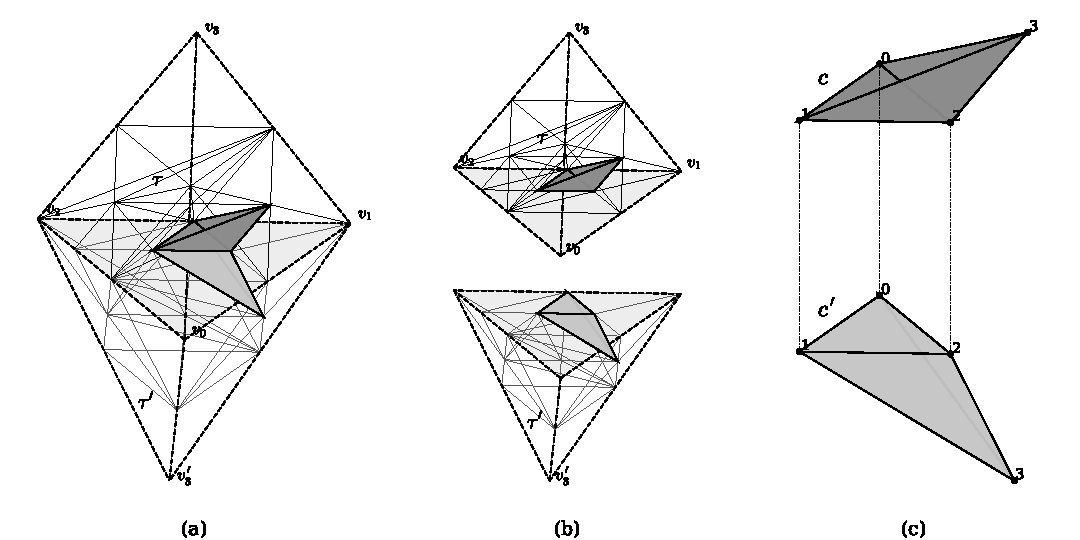
\includegraphics[width=\linewidth]{figures/seed_crossing.pdf}
\caption{Propositions~\ref{prop:boundary-test} and~\ref{prop:crossing} in
dimension $3$. (a)~Two colour-ordered seed tetrahedra $\tau$ and $\tau'$,
glued along their common facet $\langle v_0,v_1,v_2\rangle$ (light grey),
after adaptive Maubach bisection towards a point just above that facet.
The conforming closure propagates across the seed boundary. Dashed
lines are the seed edges. (b)~The same mesh, exploded along the normal
of the common facet: both seed cells induce the same subdivision on it.
(c)~The highlighted leaf $c\subset\tau$, whose facet $\partial_3c$ lies on
the seed boundary, and its neighbor $c'\subset\tau'$. Both have the
same bisection code (path $010010$ from their roots), and the shared
facet occupies local positions $0,1,2$ in both. The figure is generated
by a script that asserts both facts.}
\label{fig:seed-crossing}
\end{figure}


The resulting neighbor procedure is entirely combinatorial. To find the
neighbor of $c=(s,\kappa)$ across $\partial_ic$:
\begin{enumerate}[itemsep=2pt]
\item \emph{Sibling facet.} If $\partial_ic$ is the facet created by the
  last bisection ($i=d$ for a $0$-child, $i=\type$ for a $1$-child),
  return the other child of the parent (\Cref{lem:children}).
\item \emph{Boundary test.} Otherwise, look up $(j,\delta)$ for
  $(\ell,\Pi,i)$ and check the orthant condition of
  \Cref{prop:boundary-test}.
\item \emph{Interior facet.} If the test fails, return
  $(s,\kappa')$, where $\kappa'$ is given by Atalay and Mount's Theorem~2.
\item \emph{Seed crossing.} If it succeeds, return
  $(\mathrm{adj}[s][j],\kappa)$ (\Cref{prop:crossing}). The seed adjacency
  table has $N_0\times(d{+}1)$ entries; a root cell uses it directly with
  $j=i$.
\end{enumerate}
\Cref{fig:seed-crossing} illustrates rules~2 and~4 in dimension~$3$.
Rule~2 is indispensable. Atalay and Mount's Theorem~2 describes neighbors in the infinite
Kuhn arrangement, so across a seed-boundary facet it returns a cell of
the reflected reference simplex, i.e.\ a cell with negative barycentric
weights. Such crossings are frequent: about $24\%$ of the non-sibling
facets sampled at realistic depths lie on the seed boundary.

\paragraph{Verification.}
Every returned neighbor was checked \emph{exactly}. Both cells were
written as integer barycentric weights over the $15$ global vertices of
Gaifullin's triangulation, with common denominator $2^{11}$. We then
verified that the neighbor is a different cell of the same level
containing the queried facet. The check covered $10^6$ random cells over
the whole representable depth range, $0$ to $43$, and $5$ million
neighbor queries:
\begin{itemize}[itemsep=1pt]
\item sibling: $977\,070$ queries;
\item interior: $3\,317\,979$ queries;
\item seed crossing: $704\,951$ queries.
\end{itemize}
No query failed. Away from sibling facets, the facet always sits at the
\emph{same} local index in both cells, as strong compatibility predicts.
Orientation coherence was checked on $750\,000$ sampled (cell, facet)
pairs, with no violation.

\paragraph{Comparison with the first implementation.}
Our first version used a different boundary test. It computed the full
matrix of exact barycentric weights of the facet's vertices, which costs
$O(d^2+rd)$ integer operations. It also resolved crossings geometrically:
a point slightly across the facet was located by descending the
neighboring seed's hierarchy in floating point. On $7.8$ million sampled
facets, the table-based test of \Cref{prop:boundary-test} agrees with the
weight-matrix test in every case, and the same-code rule agrees with
geometric location on all $1.4$ million crossings. Both are also faster:
$4.3$\,ns against $79$\,ns per boundary test, and $5$\,ns against
$211$\,ns per crossing. The earlier floating-point path was the only
source of discrepancies in the first implementation, at the maximum
representable depth; it is now gone. The application of
\Cref{sec:riemann} produces byte-identical output with either
implementation. Its running time is dominated by root finding on
$2$-faces, so the end-to-end speedup is small, about $2\%$.

\subsection{The leaf set and graded conforming refinement}

The mesh is the set of codes of the current leaves. They are stored in an
open-addressing hash table with one 64-bit slot per leaf, linear probing
and backward-shift deletion; the last avoids tombstones under the
constant erase-two-insert churn of bisection. For Gaifullin's seed
($d=4$, $N_0=108$), a code fits in one word:
\begin{center}
\begin{tabular}{@{}lcccccc@{}}
\toprule
field & seed & $\ell$ & $\Pi$ & $r$ & $o_1,\dots,o_4$ & total \\
\midrule
bits & 7 & 2 & 9 & 4 & $4\times10$ & 62 \\
\bottomrule
\end{tabular}
\end{center}
This allows $r\le10$ rounds, i.e.\ depth $43$.

Two operations sit on top of this table.
\begin{itemize}[itemsep=2pt]
\item $\texttt{compat\_bisect}(c)$ is \Cref{alg:maubach} expressed on
  codes. Before bisecting $c$, it recursively bisects coarser neighbors, so
  that the mesh stays graded: no facet separates cells more than one level
  apart.
\item $\texttt{neighbor\_leaf}(c,i)$ walks up the ancestor chain of the
  combinatorial neighbor until it finds a current leaf. If the neighbor
  has been refined further than $c$, it reports this instead.
\end{itemize}
An exhaustive graded-invariant test checked about $40\,000$ cascading
bisections producing roughly $4$ million leaves, $11.6$ million facet
checks in total, with no violation.

Vertex identities and coordinates are not part of the code. When a cell
is created, its new vertex receives a global integer identifier, keyed by
the identifiers of the endpoints of the split edge in a separate hash
table. Coordinates are attached to vertex identifiers only. Vertices are
far fewer than cells: about $1/d!$ per cell asymptotically.

\paragraph{Limitations.}
\texttt{glpt} does not yet enumerate the several finer leaves that may
border a coarser facet. Such queries are reported, never guessed. For
seeds that are compatible only in the weak sense of (MaubachA), with the
$\{0,\type\}$ exception, the two identifications disagree on shared
facets, and \Cref{prop:crossing} would need a permutation correction.
For seeds initialized as in~\cite{dgs2025} with $N>d$ colors, a cell is a
face of a virtual $N$-simplex. Its code would live in the $N$-dimensional
reference hierarchy, but~\cite[Rem.~12]{dgs2025} shows that refinements
of the virtual extension do not restrict to refinements of the mesh. We
leave both cases open.

% =====================================================================
\section{Application: Riemann surfaces in $\CP^2$}
\label{sec:riemann}
% =====================================================================

\subsection{Setting}

Let $F(X,Y,Z)$ be a homogeneous polynomial of degree $n$ defining a smooth
curve $C=\{F=0\}\subset\CP^2$. $C$ is a compact Riemann surface of genus
$(n-1)(n-2)/2$, a real surface of codimension $2$ in the real $4$-manifold
$\CP^2$. We triangulate $C$ in three steps:
\begin{enumerate}[itemsep=1pt]
\item mesh $\CP^2$ adaptively, starting from Gaifullin's triangulation
  realized with its explicit coordinates~\cite{gaifullin2009};
\item refine by pointerless Maubach bisection (\Cref{sec:lpt}), placing
  each new vertex at the \emph{Fubini--Study geodesic midpoint} of the
  split edge;
\item extract $C$ cell by cell.
\end{enumerate}
The resulting cells are not affine simplices in any chart. Their vertices
are points of $\CP^2$ and their $2$-faces are handled in the
best-conditioned affine chart of each face. Midpoints are computed after
aligning the phases of the two homogeneous representatives. Because the
geodesic midpoint does not commute with linear combinations, vertex
coordinates are threaded along the bisection path from the root, cached by
global vertex identifiers.

To avoid resonance between the curve and the seed's coordinate axes, the
seed may be moved by a random unitary change of basis of $\C^3$.

\subsection{Per-cell extraction}

For a leaf $c$, each of its $10$ triangular $2$-faces is intersected with
$C$ by Newton's method in barycentric coordinates, from several seeds.
Solutions are cached by the sorted triple of global vertex identifiers, so
that neighboring cells see identical crossing points.
Generically $C$ meets a $2$-face transversally in isolated points. The
crossing points of the $5$ tetrahedral facets of $c$ are paired into arcs
(by minimal total geodesic length when a facet has four crossings). The
resulting graph is decomposed into closed polygons approximating
$C\cap c$. A cell is \emph{bad} when this decomposition fails: a node of
degree $\ne2$, or three crossings on one facet.

An optional mode encloses $F$ on a $2$-face using its Bernstein--Bézier
coefficients on the triangle, in the spirit of~\cite{reuter2008}. It is
used to certify empty faces and to recover roots missed by Newton.

\subsection{Continuation}

\Cref{alg:continuation} follows the curve from a single cell it is known
to meet. Only the combinatorial operations of \Cref{sec:lpt} are used to
move through the mesh.

\begin{algorithm}[t]
\caption{Continuation triangulation of $C=\{F=0\}$}
\label{alg:continuation}
\begin{algorithmic}[1]
\Require balanced seed $T$ (as a \texttt{glpt} leaf set); curve $F$; target depth $D$
\State $s\gets$ first seed cell whose extraction finds a crossing
\State $\mathit{visited}\gets\varnothing$; $\mathit{frontier}\gets\{s\}$
\While{$\mathit{frontier}\neq\varnothing$}
  \State pop $c$; \textbf{skip} if $c\notin T$ or $c\in\mathit{visited}$
  \State $\mathit{visited}\gets\mathit{visited}\cup\{c\}$; $r\gets\mathrm{extract}(c)$
  \State \textbf{skip} if $r$ has no crossing
  \If{$\level(c)<D$}
    \State $T.\texttt{compat\_bisect}(c)$; add the newly created leaves to $\mathit{frontier}$
  \Else
    \State record $r$
    \For{$i=0,\dots,4$}
      \State \textbf{if} $T.\texttt{neighbor\_leaf}(c,i)$ finds $n\notin\mathit{visited}$ \textbf{then} add $n$ to $\mathit{frontier}$
    \EndFor
  \EndIf
\EndWhile
\end{algorithmic}
\end{algorithm}

If $C$ crosses a facet shared by cells $A$ and $B$, it also meets $B$, so
propagation through crossing facets reaches every cell met by the
connected curve. Reducible curves need one seed per component.

Two refinement mechanisms act beyond the target depth.
\begin{itemize}[itemsep=2pt]
\item \emph{Proactive: tangency threshold.} At each crossing, let $w_k$ be
  the complex directional derivatives of $F$ along the two edge vectors
  $e_1,e_2$ of the $2$-face, and $(F_a,F_b)$ its chart gradient. By the
  Cauchy--Riemann equations, the quantity
  \[
    \mathrm{score}=\frac{|\mathrm{Im}(\overline{w_1}w_2)|}{|e_1||e_2|(|F_a|^2+|F_b|^2)}\in[0,1]
  \]
  vanishes exactly when the face is tangent to $C$ at the crossing. Cells
  whose minimal score falls below a threshold are bisected further, within
  an extra depth budget.
\item \emph{Reactive: repair rounds.} Bad cells are re-bisected and
  re-extracted.
\end{itemize}

\subsection{Results}

We tested six smooth curves: a conic, the Fermat cubic, a generic
Hesse-pencil cubic, a smooth quartic, a parabola and an elliptic curve.
Continuation recovers exactly the same leaf set and the same bad cells as
a global scan of all $108$ seed hierarchies with the same test, at depths
$8$, $12$ and $14$. Compared with the earlier refinement criterion based
on gradient dispersion, which refines all of $\CP^2$, continuation yields
meshes $3$ to $6$ times smaller at depth $14$. Its bad-cell rate is never
worse.

For the elliptic curve $X^2Z-Y^3+YZ^2=0$, with a random unitary rotation
of the seed:
\begin{center}
\small
\begin{tabular}{@{}llrrrr@{}}
\toprule
depth & mode & leaves & good cells & bad cells & bad rate \\
\midrule
14 & baseline & 327\,370 & 27\,397 & 887 & $3.14\%$ \\
14 & repair rounds (2) & 327\,370 & 30\,605 & 730 & $2.33\%$ \\
14 & tangency threshold $0.05$ & 612\,978 & 42\,278 & 904 & $2.09\%$ \\
14 & both & 612\,978 & 45\,709 & 729 & $1.57\%$ \\
\midrule
20 & baseline & 4\,620\,102 & 222\,981 & 1\,348 & $0.601\%$ \\
20 & repair rounds (2) & 4\,678\,426 & 226\,677 & 678 & $0.298\%$ \\
20 & tangency threshold $0.05$ & 6\,788\,844 & 335\,517 & 1\,260 & $0.374\%$ \\
20 & both & 6\,842\,524 & 339\,147 & 610 & $\mathbf{0.180\%}$ \\
\bottomrule
\end{tabular}
\end{center}

At depth $20$ (baseline), we evaluated $|F|$ at the $164\,390$ distinct
extracted vertices, with unit-norm homogeneous representatives. The median
is $1.0\times10^{-16}$, the $99$th percentile $4.3\times10^{-13}$ and the
maximum $9.8\times10^{-13}$.

Instrumenting the extraction at depth $14$ ($136\,786$ touched cells over
all six curves, $8.0\%$ bad) attributes the failures to near-tangency:
\begin{itemize}[itemsep=1pt]
\item $82\%$ of the bad cells fail on node degree, $18\%$ on facets with
  three crossings;
\item cells containing a facet touched at a single point are $7$ times
  more likely to be bad;
\item the tangency score separates good cells (median $0.21$) from bad
  ones (median $0.12$), with a monotone gradient in bad rate across score
  buckets.
\end{itemize}
Bisection with Fubini--Study midpoints splits cell volumes unevenly, but
this imbalance does \emph{not} correlate with bad cells.

\begin{figure}[t]
\centering
\begin{minipage}[b]{0.50\linewidth}\centering
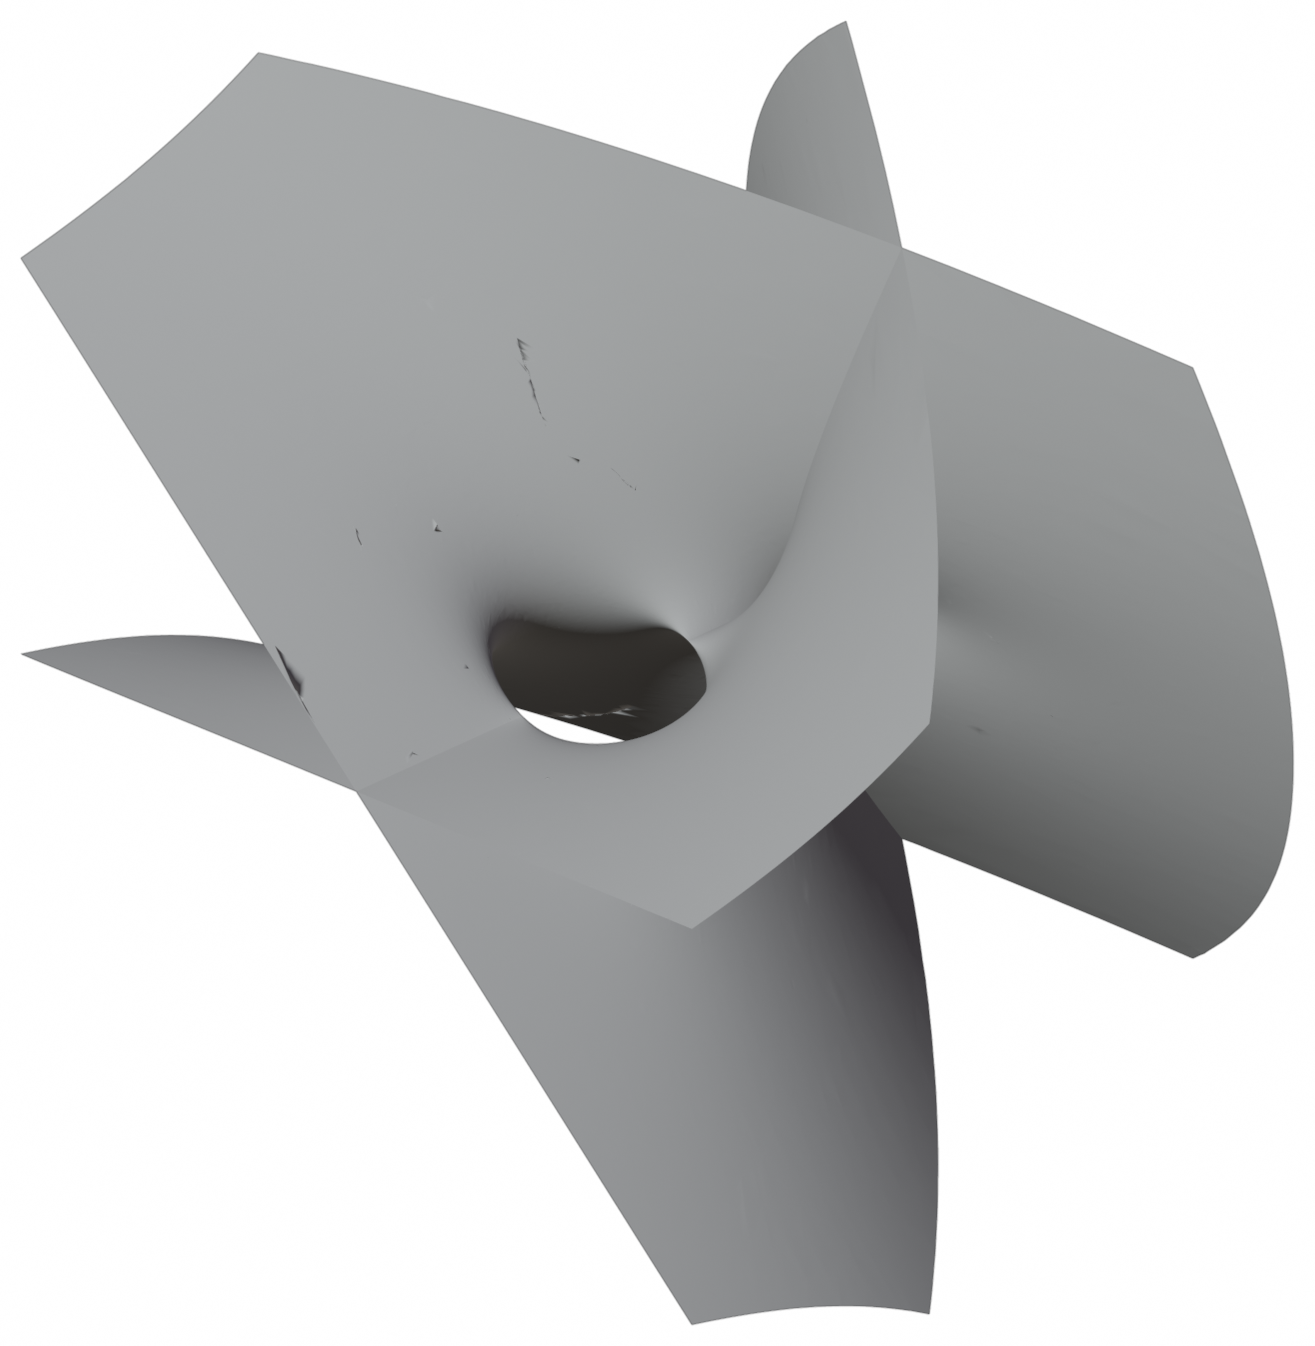
\includegraphics[width=\linewidth]{figures/elliptic_flat.png}\\[2pt]
{\small (a)}
\end{minipage}\hfill
\begin{minipage}[b]{0.40\linewidth}\centering
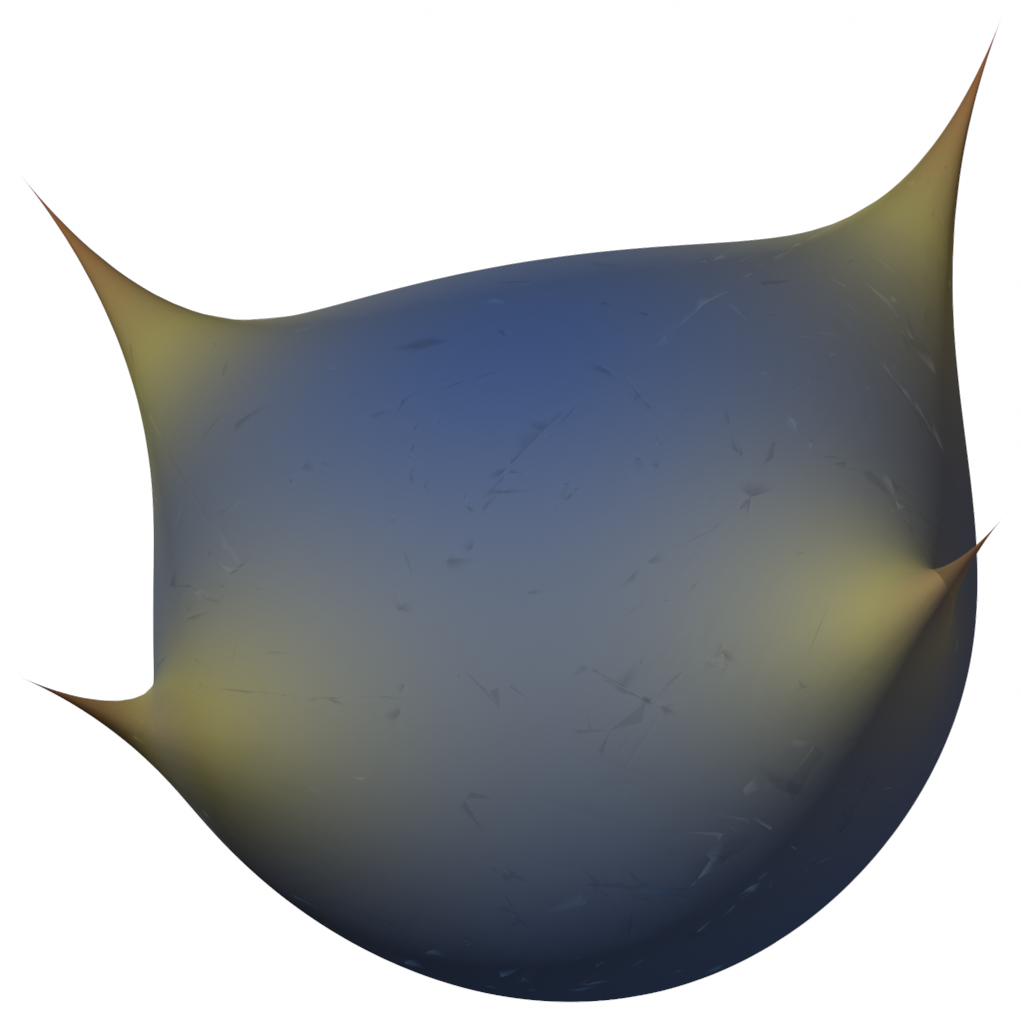
\includegraphics[width=\linewidth]{figures/quartic_alpha.png}\\[2pt]
{\small (b)}
\end{minipage}
\caption{Riemann surfaces triangulated intrinsically in $\CP^2$ by
\Cref{alg:continuation}.
(a)~The elliptic curve $X^2Z-Y^3+YZ^2=0$, i.e.\ $w^2=z^3-z$ in the chart
$Z=1$ with $w=X$ and $z=Y$, shown as the classical graph
$(\mathrm{Re}\,z,\mathrm{Im}\,z,\mathrm{Re}\,w)$, clipped to
$|\mathrm{Re}\,z|,|\mathrm{Im}\,z|\le2$ and $|\mathrm{Re}\,w|\le3$. The
two sheets meet over the branch points $z=0,\pm1$. Depth $18$ with
tangency threshold $0.05$ and two repair rounds: $3.03$M leaves,
$177\,650$ good and $701$ bad cells ($0.39\%$).
(b)~The Fermat quartic $X^4+Y^4+Z^4=0$ (genus $3$) under Dutter's
chart-free projection $\tilde\alpha:\CP^2\to\R^3$~\cite{dutter2026}.
It is coloured by distance to the centre, from blue (near) to red (far),
and drawn semi-transparent. Depth $17$, same settings: $2.40$M leaves,
$155\,436$ good and $5\,388$ bad cells ($3.35\%$).
Both surfaces were closed by the topological post-processing described
in \Cref{sec:riemann}: cones over the holes left by bad cells, with
apices on the curve. The closed complexes were verified to be closed
surfaces of the correct genus. The faint marks visible on both surfaces
are discontinuities of the interpolated normals, not holes. They occur
where the small closing cones meet the surrounding mesh (most of the
marks in~(b)), and at a few thin or slightly folded polygons produced by
the extraction itself (the darker streaks in~(a)). Rendering scripts are provided with the code~\cite{vgtl}.}
\label{fig:riemann}
\end{figure}

\Cref{fig:riemann} shows two of the resulting surfaces.

\paragraph{Topological check.}
Although the output is not certified, its topology can be checked a
posteriori, directly on the extracted complex in $\CP^2$ and independently
of any projection. Output vertices are identified combinatorially: a
crossing is keyed by the mesh vertex, edge or $2$-face it lies on. The
extracted polygons therefore form a single $2$-complex. Each bad cell
leaves a hole. A hole is a loop of edges that belong to a single
polygon. A vertex is \emph{pinched} if its link has more than one component;
we split every pinched vertex into one copy per link component. In all
our runs, every pinched vertex lies on hole boundaries: its link consists
of exactly two paths. About two thirds are points where the outline of
a single hole touches itself; the rest are points where two holes meet.
We never observed two sheets touching in the interior. If the
remaining holes are discs, the resulting surface with $c$ components and
$b$ boundary loops satisfies
\[
  \chi=\sum_{i=1}^{c}(2-2g_i)-b,
  \qquad\text{hence}\qquad
  g=\sum_i g_i=\frac{2c-b-\chi}{2}.
\]
The estimate recovers the genus $(n-1)(n-2)/2$ exactly in every case we
tried, even at a bad-cell rate close to $6\%$:
\begin{center}
\small
\begin{tabular}{@{}lrrrrrrrr@{}}
\toprule
curve & depth & bad cells & pinched & $c$ & $b$ & $\chi$ & $g$ est. & $g$ \\
\midrule
conic $XY-Z^2$ & 14 & $367$ ($1.2\%$) & 3 & 2 & 41 & $-37$ & 0 & 0 \\
elliptic $X^2Z-Y^3+YZ^2$ & 14 & $729$ ($1.6\%$) & 8 & 4 & 84 & $-78$ & 1 & 1 \\
elliptic, Fig.~\ref{fig:riemann}(a) & 18 & $701$ ($0.39\%$) & 3 & 2 & 104 & $-102$ & 1 & 1 \\
Fermat cubic & 14 & $2\,438$ ($5.9\%$) & 35 & 8 & 253 & $-239$ & 1 & 1 \\
Fermat quartic & 17 & $5\,388$ ($3.4\%$) & 36 & 11 & 656 & $-640$ & 3 & 3 \\
\bottomrule
\end{tabular}
\end{center}
All runs use a random unitary rotation of the seed, tangency threshold
$0.05$ and two repair rounds. That the check succeeds shows that the
failures are local: each hole is a disc, and no hole cuts through a
handle of the surface.

\paragraph{Topological closing.}
The same analysis yields a simple post-processing step that turns the
extracted complex into a closed surface of the correct topology:
\begin{enumerate}[itemsep=1pt]
\item split the pinched vertices as above;
\item keep the main connected component. The splitting cuts off a few
  tiny islands, from $1$ to $18$ faces in our runs, which lay inside a
  hole whose outline touched itself;
\item cap every boundary loop by a cone from a \emph{new} apex vertex.
  A fan from an existing vertex of the loop could duplicate an edge that
  already exists in the mesh. The apex is placed at the Fubini--Study
  barycentre of the loop and moved onto the curve by Newton's method in
  the best affine chart (minimum-norm steps for one complex equation in
  $\C^2$);
\item verify the result: every edge lies in exactly two faces, every
  vertex link is a single cycle, the complex is connected, and
  $\chi=2-2g$ with $g=(n-1)(n-2)/2$.
\end{enumerate}
The last step makes the procedure self-certifying with respect to
topology: a hole that was not a disc would change $\chi$ and be
detected. On all the runs of the previous table, the closed surface
passes every check: the conic gives $\chi=2$, the cubics $\chi=0$,
and the quartic $\chi=-4$. In every case, Newton's method moved every
cone apex onto the curve. Being topological, the procedure acts on the
complex in $\CP^2$ and is independent of the projection later used for
display. The surfaces of \Cref{fig:riemann} are closed this way.

\paragraph{Bad-cell rate versus depth.}
\Cref{fig:badrate} shows how the bad-cell rate evolves with the
refinement depth for four curves of degree $2$ to $4$. The rate
decreases steadily, roughly halving every two levels. The proactive
tangency threshold combined with repair rounds lowers it by a factor of
$1.5$ to $3$ at every depth. Curves of higher degree need a few more levels to reach the same
rate.

\begin{figure}[t]
\centering
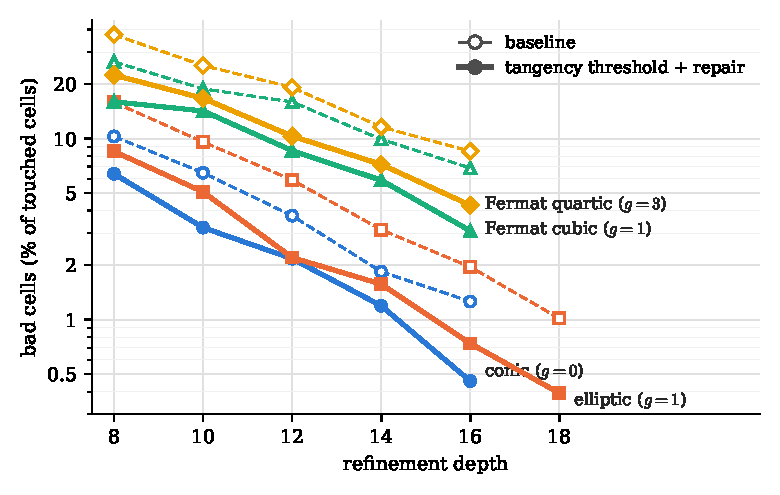
\includegraphics[width=0.78\linewidth]{figures/badrate.pdf}
\caption{Percentage of touched cells whose extraction fails, against the
refinement depth, for four smooth curves (seed rotated by the same random
unitary change of basis). Dashed lines with open markers: continuation
alone. Solid lines: with tangency threshold $0.05$ and two repair rounds.
The elliptic curve is also shown at depth $18$, the mesh of
\Cref{fig:riemann}(a). Data and scripts are provided with the
code~\cite{vgtl}.}
\label{fig:badrate}
\end{figure}

\subsection{Discussion}

Four features distinguish the construction from chart-based approaches.
\begin{itemize}[itemsep=2pt]
\item \emph{Intrinsic.} $\CP^2$ is compact and the seed is symmetric under
  a group of isometries, so there are no charts, branch cuts or special
  points at infinity. Local affine charts appear only inside the numerical
  solve on a single $2$-face.
\item \emph{Codimension two.} The extraction runs directly in the real
  4-manifold, as in~\cite{weiglebanks1996}, but on an adaptive mesh.
\item \emph{Combinatorial navigation.} The neighbor structure of the
  pointerless mesh is all the continuation needs. Memory is proportional
  to the number of leaves, which allowed depth $20$ with close to $7$
  million leaves on a workstation with 7.2\,GB of RAM.
\item \emph{Not certified.} Unlike~\cite{plantingavegter2004,bkw2023},
  the output is not guaranteed to be isotopic to $C$. The residual bad
  cells, concentrated at near-tangencies, are the price. Their effect is
  purely local, however: after topological closing, the result is a
  closed surface whose genus is verified to be correct.
\end{itemize}
A certified variant would combine the Bernstein enclosures with a
transversality test on each $2$-face. We leave this for future work.

% =====================================================================
\section{Conclusion}
% =====================================================================

Stellar subdivision schemes reduce the correctness of Maubach bisection to
three local lemmas about ordered stellar operations. On conforming
meshes, the strong form of the invariant is precisely balance. This single
notion explains:
\begin{itemize}[itemsep=1pt]
\item the classical constructions (products of simplices and barycentric
  subdivisions);
\item the coloring-based initializations of the finite-element
  literature;
\item the portability of pointerless LPT codes to arbitrary seeds.
\end{itemize}
Balanced triangulations of closed manifolds become natural seeds. For
$\CP^2$, Gaifullin's triangulation is a vertex-minimal balanced one. On
top of it, pointerless Maubach bisection and combinatorial continuation
triangulate Riemann surfaces intrinsically in $\CP^2$.

Several questions remain open:
\begin{itemize}[itemsep=1pt]
\item a precise dictionary between (MaubachA) and Stevenson's matching
  condition;
\item pointerless codes for weakly compatible seeds, and for the $N>n$
  initializations of~\cite{dgs2025};
\item a systematic search for small balanced triangulations of other
  closed manifolds, for example with the tools of~\cite{venturello2019};
\item Gaifullin's $33$-vertex subdivision, on which the moment map is
  simplicial, as an alternative seed;
\item certification of the extraction.
\end{itemize}

\section*{Note on AI assistance}
The implementation described here was developed with Claude (Anthropic)
acting as a coding assistant, under the author's direction, review and
testing. The software comprises the \texttt{glpt} pointerless mesh, the
continuation algorithm and the diagnostic measurements. This draft was
likewise prepared with Claude's assistance.
\paragraph{Code availability.}
The ordered-mesh data structures and the stellar subdivision algorithms,
including the Mitchell and Maubach schemes and the Riemann-surface
programs of \Cref{sec:riemann}, are part of VGTL~\cite{vgtl}. The LPT
codes and their \texttt{glpt} extension to balanced seeds, with the test
suites used in \Cref{sec:lpt}, are in the \texttt{lpt}
repository~\cite{lptcode}.

\paragraph{Funding.} This research received no specific funding.

\bibliographystyle{plain}
\bibliography{related_work}

\end{document}
